%\documentclass[a4paper,norsk,12pt]{article}
\documentclass[a4paper,12pt]{article}

\usepackage{fancyhdr}
\setlength{\headheight}{15.2pt}
\pagestyle{fancy}
\setlength{\parindent}{0in} % Setter lengden på det automatiske innrykket for hver paragraf

\usepackage[utf8]{inputenc} % Tegnsett UTF-8.
\usepackage[T1]{fontenc,url}
% \usepackage[norsk]{babel} % Norsk språkpakke.
\usepackage[table]{xcolor}
\usepackage{setspace}
\usepackage{subfigure}
\onehalfspacing

\usepackage{amsmath}

\usepackage{float}

\headwidth = 390pt
\textwidth = 390pt

\usepackage{lastpage}
% \cfoot{Side \thepage\ av \pageref{LastPage}}
% \cfoot{}

\usepackage[bottom]{footmisc} % Tvinger alle footnotes nederst på siden

% Forside-stuffs
\usepackage[pdftex]{graphicx}
\newcommand{\HRule}{\rule{\linewidth}{0.5mm}}

\lhead{Architectural description} % venstrestilt header
\rhead{Page \thepage\ of \pageref{LastPage}} % høyrestilt header

\usepackage[pdfborder={0 0 0}]{hyperref}

\title{Architectural description}
\author{Steinar Haram}

\begin{document}

\begin{titlepage}

\begin{center}

\textsc{\Large TDT4240}\\[1.0cm]

\textsc{\LARGE Software Architecture}\\[1.0cm]

\textsc{\Large Spring 2012}\\[1.0cm]

\textsc{Group A17} \\
\textsc{Android SDK}


\includegraphics[width=240pt]{./androids}\\[0.5cm]   

% Participants
\begin{minipage}{0.4\textwidth}
\begin{flushleft} \large

Steinar \textsc{Haram}\\
Emil Andreas \textsc{Mork}\\

\end{flushleft}
\end{minipage}
\begin{minipage}{0.4\textwidth}
\begin{flushright} \large

Stian \textsc{Sørebø}\\
Ole Jørgen \textsc{Rishoff}

\end{flushright}
\end{minipage}\\[1.0cm]

% Document title
\HRule \\[0.4cm]
{ \huge \bfseries Requirement Document v1.0}\\[0.4cm]
\HRule \\[1.5cm]

% Focuses
\begin{minipage}{0.4\textwidth}
\begin{flushleft} \large

\textsc{Primary focus:}\\
\textsc{Maintainability}\\

\end{flushleft}
\end{minipage}
\begin{minipage}{0.4\textwidth}
\begin{flushright} \large

\textsc{Secondary focus:}\\
\textsc{Usability}

\end{flushright}
\end{minipage}

\vfill

\end{center}

\end{titlepage}


\tableofcontents
\listoftables
\listoffigures


% \caption[list-of-figure text]{actual caption text}

\pagebreak
\section{Introduction}

This document contains implementation details for our developed version of the classical \emph{Nine Men's Morris} game. The game is developed as a native Android application. The applications primary attribute is modifiability, while its secondary attribute is usability. The second chapter will highlight the design and implementation details. The following chapter contains a user manual, while chapter four contains a brief description of the testing of functional and quality requirements. The relation between the implementation and the planned architecture will be reviewed in chapter five. IChapter six highlights encountered problems and gained experience.





\section{Design and implementation details}

{\bf Here you describe a more detailed view of the various parts of the architecture describing how the robot controller or game was designed.}


\subsection{Skiller multiplayer framework}
Due to the desire of developing a fully functional multiplayer game, the \emph{Skiller multiplayer framework} \cite{skiller} has been used. This is a third party COTS software, and its usage has sped up the development process. Registration was needed in order to gain access to the Skiller SDK. When the registration was done, a new game could be created, and an application ID, an application key, and an application secret was supplied. These are used in the code to identify the specific application. \\

This framework supplies a server solution for turn based games, and it has been implemented in the network class. When playing a network game, the GameController class tells the Game model to  network class sends event messages to the server, and the server delivers it to the opponent.

\subsection{Activities}
Figure \ref{fig:activities} shows an overview of the application's different activities, and how the user interactions can change them. The user can navigates back to the menuActivity by pressing the back button.\\

\begin{figure}[H]
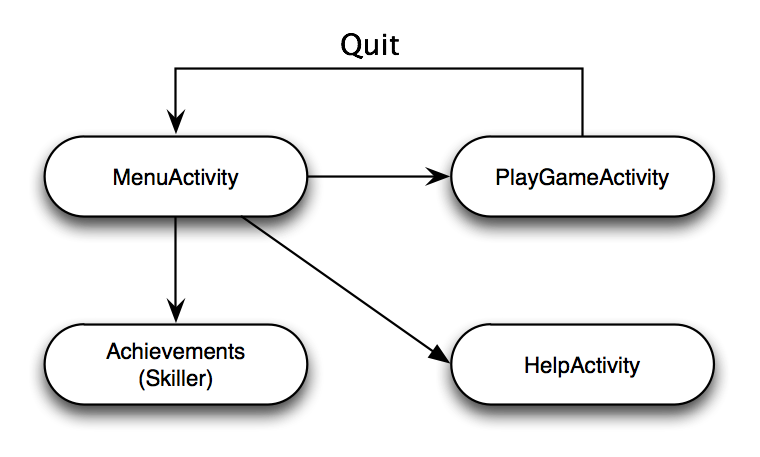
\includegraphics[width=1\textwidth]{Images/activities}
\caption{Application activities}
\label{fig:activities}
\end{figure}

The MenuActivity shows a menu consisting of five items, allowing the user to create or join a multiplayer game, start a local game, check achievements, or check the game rules. The PlayGameActivity is responsible for creating or joining multiplayer games, and starting local games. The HelpActivity is responsible for showing the game rules. The achievement screen is supplied by \emph{Skiller}.\\

Screencaps of the different activities, and the achievement screen, are shown in section \ref{section:playing}.
%\ref{section:label}

\subsection{MVC}

Our implementation of the MVC structure is based interface communication. In regular java there is more common to create a MVC structure where the view has model and the controller contains view and model. Android has its own MVC structure where an activity represent controller and view, which make it difficult to build ut the MVC on the regular way. The most favorable way of createing MVC in android is to use interfaces to update the view when there are changes in the model. Figure~\ref{fig:mvc} is a excerpt from our class diagram that shows our MVC structure with BoardView(View), GameController(Controller) and Game(Model). When the user interact with the ciew the controller handles the user action and tell the model what to do. When the model is updated the view receive a message on the interface, and finally update the screen.


\begin{figure}[H]
\begin{center}
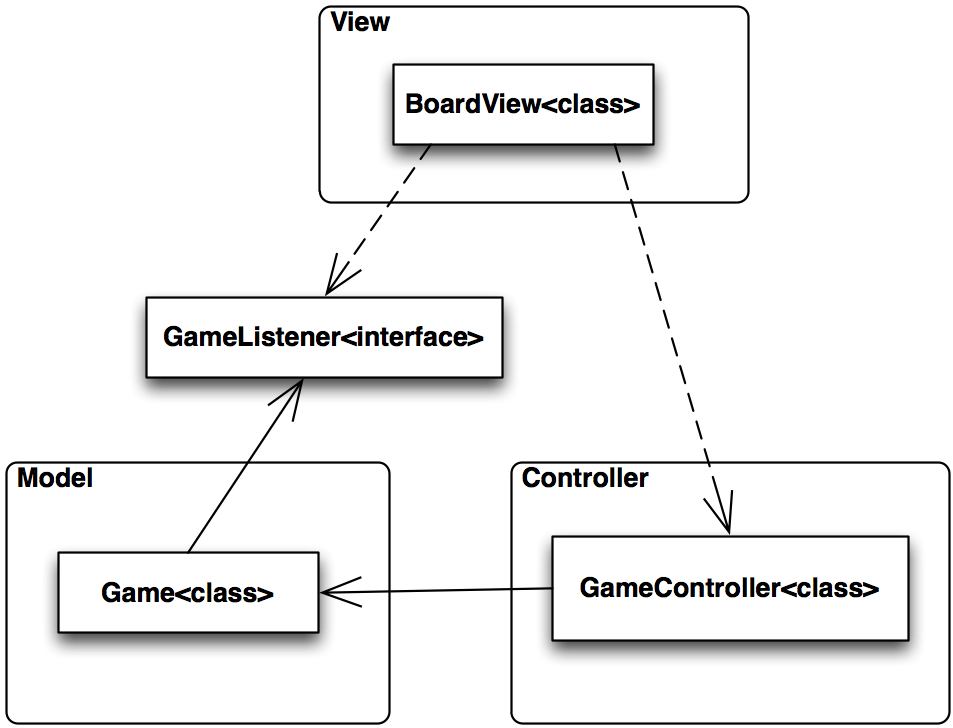
\includegraphics[width=0.7\textwidth]{Images/mvc}
\caption{MVC structure}
\label{fig:mvc}
\end{center}
\end{figure}







\section{User manual}

\subsection{Functional requirements}
\begin{itemize}
\item Requires the user to have an Android device with Android OS v2.2 or newer.
\item Requires internet connection to be able to play online.
\end{itemize}

\subsection{Running the application}
The project files are supplied with the delivery. The project can be run in an emulator or on an Android device. In both scenarios it is recommended to open the project in Eclipse. It can also be installed directly on an Android device with the supplied *.apk file.

\subsubsection{Opening project in Eclipse}
Opening the project in Eclipse is done as follows:
\begin{enumerate}
\item Choose \emph{File}
\item Choose \emph{Open project}
\item Choose \emph{Existing source code}
\item Navigate to the download path, and open the project
\end{enumerate}
%File -> Open project -> Existing source code -> path to downloaded project.

\subsubsection{Running}
To run the project in an emulator, the user needs to install an AVD, and then choose to run the project with this AVD.

\subsubsection{Running on device}
The user needs to connect the Android device to the computer, and run the project with the device set as target.

\subsubsection{Installing APK-file}
The user needs to connect the Android device to the computer, and transfer the APK-file to the SD card. The settings on the device must be set to accept installing applications from unknown sources. The next step is to open the file browser on the device, and click the application file on the SD card. It will then prompt the user to install the application.

\subsection{Game rules}
The game is implemented with the same set of rules as the classic board game \emph{Nine Men's Morris} \cite{morris}. The goal of the game is to either block any opponent moves, or to reduce your opponent's piece number to less than three. If you get three pieces in a row, you enter a morris state, and are allowed to remove one of your opponent's pieces. Pieces that are in a morris state, i.e. forms three in a row either horizontally or vertically, are not removable.

\subsection{Creating Skiller account}
When running the application, the user is prompted to create a Skiller user account. The registration only requires a username and a password. If the user already has an account, he can log in with the existing user information. The account automatically gets 50 coins that are used for playing online games in the future.

\subsection{How to play}
\label{section:playing}

\subsubsection{Choosing game mode}
A user can choose between online mode or hotseat mode. Clicking "Crate Game" or "Join Game" will start a game in online mode. Clicking "Hotseat" will start a game in hotseat mode.
\label{section:game_mode}
\begin{figure}[H]
	\centering
	\mbox{
	\subfigure[Available game modes]{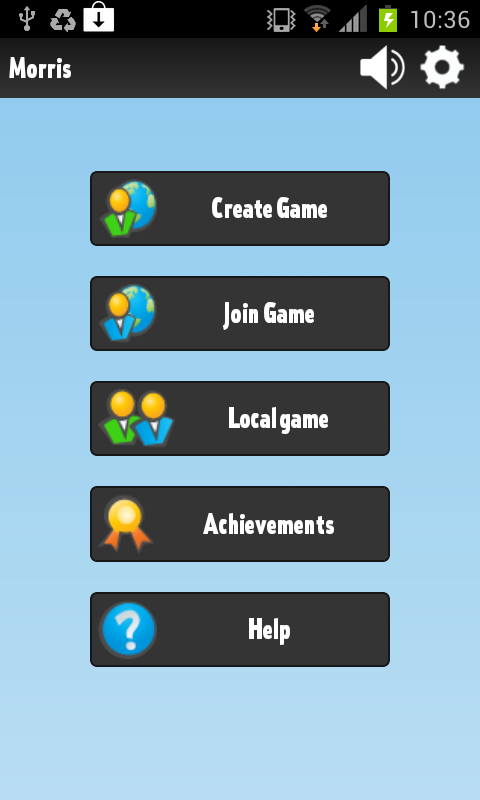
\includegraphics[width=0.3\textwidth]{Images/menuPage.png}}
	\subfigure[Achievements]{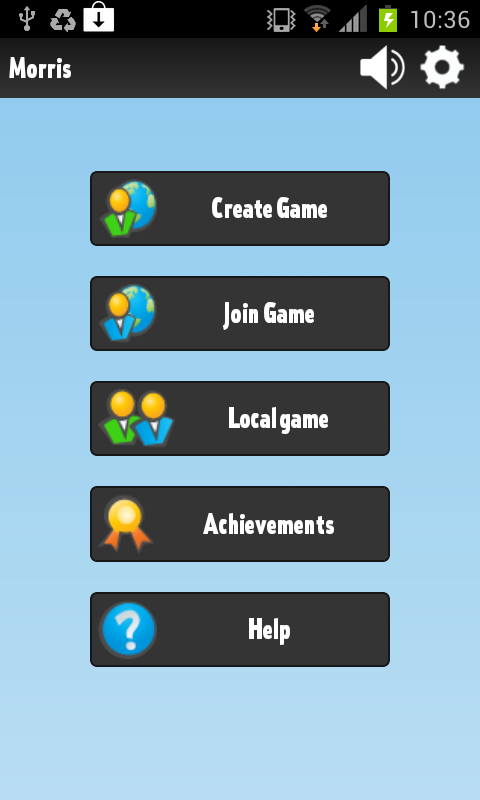
\includegraphics[width=0.3\textwidth]{Images/menuPage.png}}
	\subfigure[Help explaining the games rules]{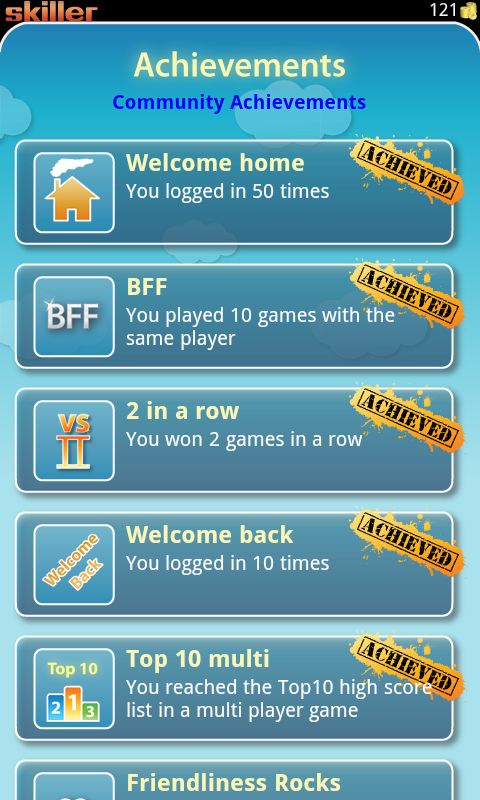
\includegraphics[width=0.3\textwidth]{Images/achievements.png}}
	}	
\end{figure}

\subsubsection{Placing, selecting, moving, and removing pieces}
When it is your turn to move, either the board or your pieces will be highlighted. In addition, the name of the current player will be blinking as the game progresses. \\
\begin{figure}[H]
	\centering
	\mbox{\subfigure[Green indicator shows where you can place a piece]{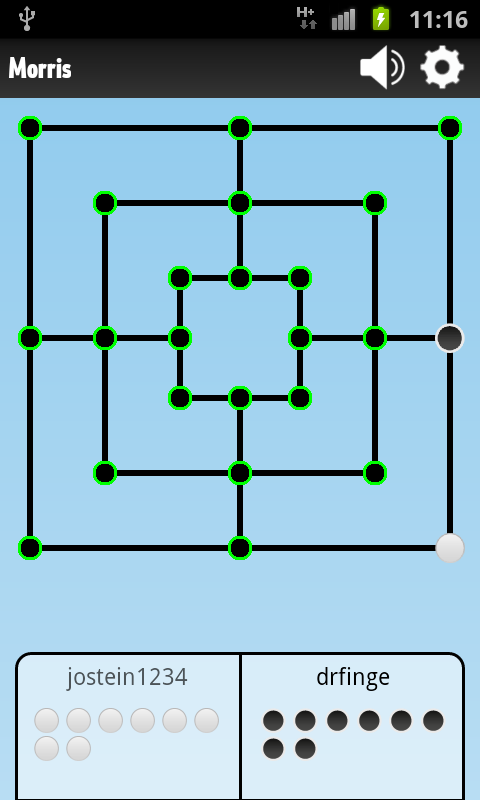
\includegraphics[width=2.1in]{Images/placementState.png}} \qquad
	\subfigure[Highlights selectable pieces]{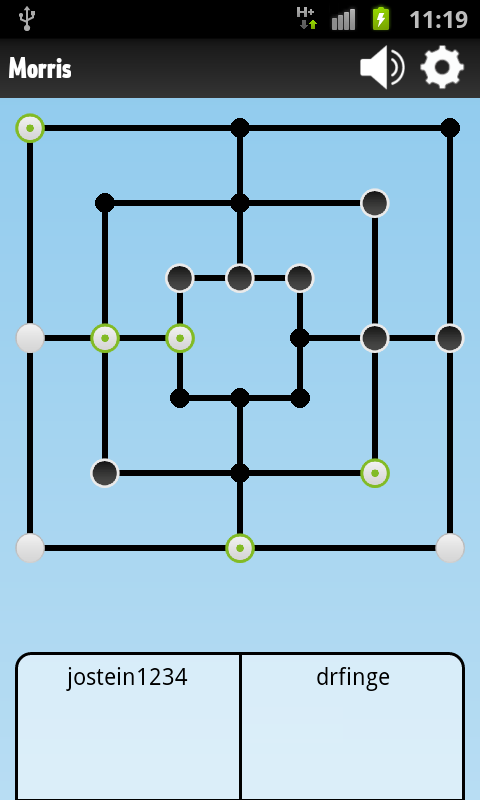
\includegraphics[width=2.1in]{Images/selectState.png}}}
	\mbox{\subfigure[Highlight selected piece, green indicator on possible moves]{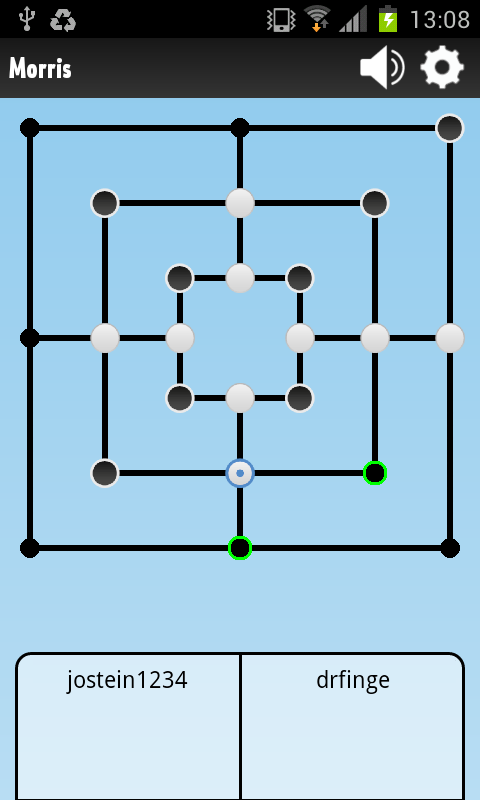
\includegraphics[width=2.1in]{Images/selectedPiece.png}} \qquad
	\subfigure[Highlights removable pieces with a red cross]{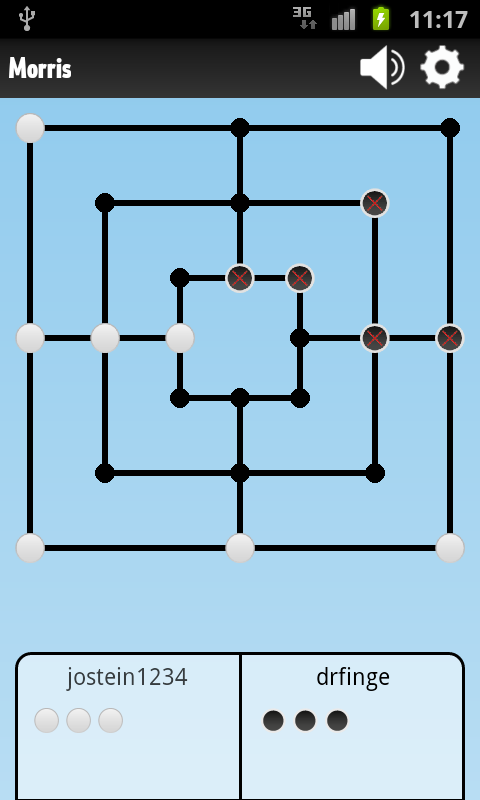
\includegraphics[width=2.1in]{Images/removalState.png}}}
\end{figure}

\subsubsection{Hotseat mode}

If you start a local game as described in section \ref{section:game_mode}, you can control both players from the same device.

\subsubsection{Online mode}

If you start an online game as described in section \ref{section:game_mode}, you are taken to the board screen, and need to wait for another player to join your game. The guest, i.e. the one who joins the game, will get the initial move. Your own pieces will always be white.







\section{Test report}

The report should contain test reports for both functional requirements and quality requirements (quality scenarios).

\subsection{Functional requirements testing}

\begin{table}[H]
\begin{tabular}{| p{100pt} | p{290pt} |} \hline
\multicolumn{2}{| l |}{FR1 - Placement of pieces} \\ \hline
Executor & Ole Jørgen Rishoff \\
Date & 12.04.2012 \\ 
Time used & 5 minutes \\ 
Evaluation & The players successfully placed all nine pieces. \\ \hline
\end{tabular}
\caption{Testing of FR1}
\end{table}

\begin{table}[H]
\begin{tabular}{| p{100pt} | p{290pt} |} \hline
\multicolumn{2}{| l |}{FR2 - Moving pieces} \\ \hline
Executor & Ole Jørgen Rishoff \\
Date & 12.04.2012 \\ 
Time used & 3 minutes \\ 
Evaluation & The players successfully moved their pieces one length at the time. \\ \hline
\end{tabular}
\caption{Testing of FR2}
\end{table}

\begin{table}[H]
\begin{tabular}{| p{100pt} | p{290pt} |} \hline
\multicolumn{2}{| l |}{FR3 - Morris state} \\ \hline
Executor & Ole Jørgen Rishoff \\
Date & 12.04.2012 \\ 
Time used & 3 minutes \\ 
Evaluation & When placing three pieces in a row, the game successfully changed state, and a piece was removed from the opponent. \\ \hline
\end{tabular}
\caption{Testing of FR3}
\end{table}

\begin{table}[H]
\begin{tabular}{| p{100pt} | p{290pt} |} \hline
\multicolumn{2}{| l |}{FR4 - Flying pieces} \\ \hline
Executor & Ole Jørgen Rishoff \\
Date & 12.04.2012 \\ 
Time used & 3 minutes \\ 
Evaluation & When the player had three pieces left, the game successfully changed state to Flying state, and the player was allowed to move to any vacant field. \\ \hline
\end{tabular}
\caption{Testing of FR4}
\end{table}

\begin{table}[H]
\begin{tabular}{| p{100pt} | p{290pt} |} \hline
\multicolumn{2}{| l |}{FR5 - Multiplayer} \\ \hline
Executor & Ole Jørgen Rishoff \\
Date & 12.04.2012 \\ 
Time used & 10 minutes \\ 
Evaluation & Ole and Emil connected to each other via the Skiller framework, and successfully played a whole game. \\ \hline
\end{tabular}
\caption{Testing of FR5}
\end{table}

\begin{table}[H]
\begin{tabular}{| p{100pt} | p{290pt} |} \hline
\multicolumn{2}{| l |}{FR6 - Game board} \\ \hline
Executor & Ole Jørgen Rishoff \\
Date & 12.04.2012 \\ 
Time used & 1 minute \\ 
Evaluation & The game has a board conforming with the layout of \emph{Nine Men's Morris}. \\ \hline
\end{tabular}
\caption{Testing of FR6}
\end{table}

% QUALITY REQUIREMENT

%\begin{table}[H]
%\begin{tabular}{| p{100pt} | p{290pt} |} \hline
%\multicolumn{2}{| l |}{FR8 - Sound effects} \\ \hline
%Executor & Ole Jørgen Rishoff \\
%Date & 12.04.2012 \\ 
%Time used & 10 minutes \\ 
%Evaluation & IKKE IMPLEMENTERT OMG. \\ \hline
%\end{tabular}
%\caption{Testing of FR8}
%\end{table}

\begin{table}[H]
\begin{tabular}{| p{100pt} | p{290pt} |} \hline
\multicolumn{2}{| l |}{FR7 - Setting player name} \\ \hline
Executor & Ole Jørgen Rishoff \\
Date & 12.04.2012 \\ 
Time used & 5 minutes \\ 
Evaluation & A player can set his own name when creating a Skiller account. \\ \hline
\end{tabular}
\caption{Testing of FR7}
\end{table}

% QUALITY REQUIREMENT

\begin{table}[H]
\begin{tabular}{| p{100pt} | p{290pt} |} \hline
\multicolumn{2}{| l |}{FR8 - Denied Morris state} \\ \hline
Executor & Ole Jørgen Rishoff \\
Date & 12.04.2012 \\ 
Time used & 10 minutes \\ 
Evaluation &  The game automatically ends a players turn when he enters a Morris state, and all the opponents pieces also is in a Morris state\\ \hline
\end{tabular}
\caption{Testing of FR8}
\end{table}

\begin{table}[H]
\begin{tabular}{| p{100pt} | p{290pt} |} \hline
\multicolumn{2}{| l |}{FR9 - Game over} \\ \hline
Executor & Ole Jørgen Rishoff \\
Date & 12.04.2012 \\ 
Time used & 5 minutes \\ 
Evaluation & When a player has only two pieces left, or cannot move any of his or her pieces, the game successfully ends. \\ \hline
\end{tabular}
\caption{Testing of FR9}
\end{table}

\subsection{Quality requirements testing}

\begin{table}[H]
\begin{tabular}{| p{100pt} | p{290pt} |} \hline
\multicolumn{2}{| l |}{FR11 - Game over} \\ \hline
\bf Executor & Ole Jørgen Rishoff \\
\bf Date & 23.04.2012 \\ 
\bf Stimuli & Addition of a new game variant \\
\bf Expected response & The architecture should allow an easy extension to \emph{Twelve Men's Morris}. \\ 
\bf Observed response & The system is flexible and an extension can easily be added. \\
\bf Evaluation & Successful \\ \hline
\end{tabular}
\caption{Testing of M1}
\end{table}






\section{Relations to the architecture}

According to our original architectural drivers we should have quality in all parts of the architecture, not too complex architecture and fast start up. In retrospect we feel that we have achived these goals. In the start, we did not implement any of the main logic, but structures that was independent on the chosen architecture. This gave us bether time to make the main logic and our architectural pattern as good as possible.\\

We were very motivated to implement the achitecture we had decided in advance. Our first concerns war related to the MVC pattern. We have decent knowledge of Android development, and we know that implementing an MVC in a native Android application needed some extra attention. \\

The implementation is very similar to the architecture we plotted at the start of the project. One notable change is that we changed the GameHandler from our original plans, and replaced it with a GameController, which gave us our final MVC structure. This was done after receiving feedback in the ATAM exercise.


\section{Issues}

%In addition to listing problems and issues with the document or with the implementation process, this is also a spot to reflect upon the project and discuss what you would have done differently if you were to start again from scratch.

It turned out that the Skiller framework was poorly documented and it gave some unreadable exception messages. This slowed down the testing quite a bit. In addition, because we normally have only had two Android devices at our disposal, much of the testing have been done in the emulator. This is of course not very effective. Also, when running the application in the emulator and creating games, players would automatically join without user interaction. The Skiller team was unable to give us any good answers to why we experienced this problem.\\

We underestimated the importance of groupwide understanding of the framework, and the implementation should have been done collectively. As it was, we assigned one person to this task, and the rest of the group were unable to do anything with the framework in his absence. We also should  have a done a more thourogh research regarding the use of the framework and its documentation. \\

We have encountered an error while running the application, caused by an empty message from the Skiller server. This has been logged at runtime, but we have not been successful in figuring out if it was a local error or if it came from the server side. This error makes the game stop responding, and is hard to trace due to the fact that it is a periodic failure. \\

\subsection{Gained experieces}
In future projects we will spend more time researching possibilities when choosing to work with a third party framework. We did not look into the documentation of the framework before implementing it, and if we had, we would probably have chosen a different framework. We will also perform a quick search for problems related to it before making a final decision.  \\

Some members of the group went into this project with more experience than others, developing native Android applications. Due to good communication we have been able to use this experience to our advantage. \\

We have gotten a better understanding of the patterns we chose to implement. The experience of implementing a MVC pattern in a native Android application has been very useful. The state pattern and its usage was unknown for all of us, but we now have a good understanding of how it can be used. We could perhaps made this pattern a bit more clear, and assign more responsibilities to the different states.

\pagebreak
\bibliographystyle{phjcp}			
\bibliography{references}
\addcontentsline{toc}{section}{References}

\end{document}
